%%%%%%%%%%%%%%%%%%%%%%%%%%%%%%%%%%%%%%%%%%%%%%%%%%%%%%%%%%%%%%%%%%%%%%%%%%%

\documentclass{standalone}

\usepackage{amsmath}
\usepackage{mathptmx}
\usepackage{pgfplots}
\usetikzlibrary{external}
\tikzexternalize{australian-population}
\pgfplotsset{compat=1.15}

%% IEEE uses Times Roman font, so we'll default to Times.
%% These three commands make up the entire times.sty package.
\renewcommand{\rmdefault}{ptm}
\renewcommand{\ttdefault}{pcr}
\normalfont\selectfont

\begin{document}

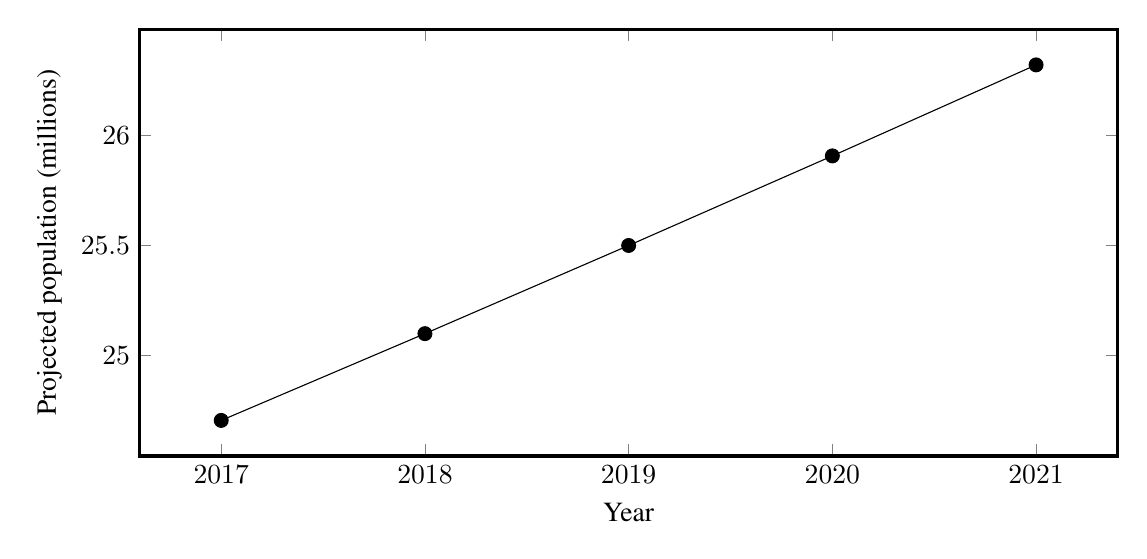
\begin{tikzpicture}
\tikzset{%%
  every mark/.append style={scale=1.0},%%
  scale=1.0%%
}
\pgfplotsset{%%
  every axis/.append style={font=\normalsize}%%
}
%%
\begin{axis}[%%
  axis line style=very thick,%%
  dotStyle/.style={mark size=2.5,black,mark color=black,mark=*},%%
  enlargelimits=true,%%
  height=7cm,%%
  plotStyle/.style={%%
    domain=4:17,%%
    mark=none,%%
    smooth,%%
    thick%%
  },%%
  width=14cm,%%
  %% x axis
  xlabel={\normalsize Year},%%
  xtick={2017,2018,2019,2020,2021},%%
  xticklabels={$2017$,$2018$,$2019$,$2020$,$2021$},%%
  %% y axis
  ylabel={\normalsize Projected population~(millions)}%%
]
%%
%%
\addplot[dotStyle] coordinates {
  (2017, 24.7029)
  (2018, 25.0981464)
  (2019, 25.4997167424)
  (2020, 25.9077122102784)
  (2021, 26.3222356056429)
};
\end{axis}
\end{tikzpicture}

\end{document}
